%\documentclass[tikz, border=5pt]{standalone}
\begin{document}
	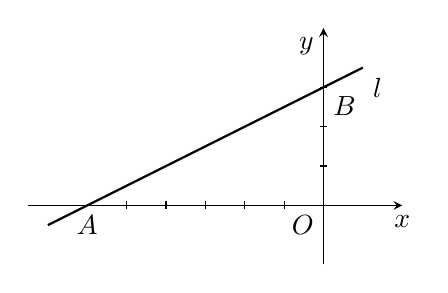
\begin{tikzpicture}[>=stealth, scale=0.5]
		% 绘制坐标轴
		\draw[->] (-7.5,0) -- (2,0) node[below] {$x$}; % x轴(带箭头和标签)
		\draw[->] (0,-1.5) -- (0,4.5) node[below left] {$y$}; % y轴(带箭头和标签)
		\node at (0,0) [below left] {$O$};           % 原点O的标签
		% 直线l  y=x/2+3
		\draw[thick] (-7, -0.5) -- (1, 3.5) node[below right] {$l$}; 
		% 绘制所有小刻度线(从 -1 到 2,每隔 1 单位画竖线)
		\foreach \x in {-5, -4,...,-1} {
			\draw (\x, 0.1) -- (\x, -0.1);  % 小竖线(长 0.2 单位)
		}
		\foreach \y in {0,1,...,3} {
			\draw (0.1,\y) -- (-0.1,\y);  % 小竖线(长 0.2 单位)
		}
		% 标记各点的标签 实心圆点
		%		\fill (G) circle (2pt) node [right] {$G$};  % 带标签的实心点
		\node at (-6,0) [below] {$A$}; 
		\node at (0,3) [below right] {$B$}; 
		
	\end{tikzpicture}
\end{document}
